  \subsection{Medición de tensión eficaz de ondas no sinusoidales}
    Haciendo uso del generador de funciones se setean señales de forma cuadrada y
    triangular de una amplitud de $5~V_{pp}$ y frecuencia de $50~Hz$. Luego, se 
    mide el valor de tensión con ambos multímetros, se calcula el error, y finalmente,
    se tabula.

    \subsubsection{En una onda cuadrada}
      En la Figura~\ref{fig:SeñalCuadrada} se puede observar la señal cuadrada seteada.
      Luego, en la Figura~\ref{fig:MedicionSeñalCuadrada} se observa la medición de tensión
      con ambos multímetros.

      \begin{figure}[H]
        \centering
        \frame{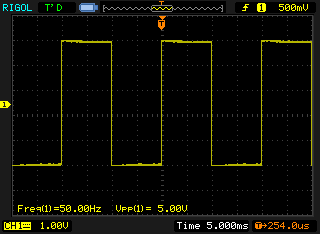
\includegraphics[width=0.48\textwidth]{Imagenes/ActividadPractica/MedicionDeTensionEficaz/Exp1_OndaCuadrada.png}}
        \caption{Señal cuadrada a medir.}
        \label{fig:SeñalCuadrada}
      \end{figure}

      \begin{figure}[H]
        \centering
        \begin{subfigure}[ht]{0.48\textwidth}
          \frame{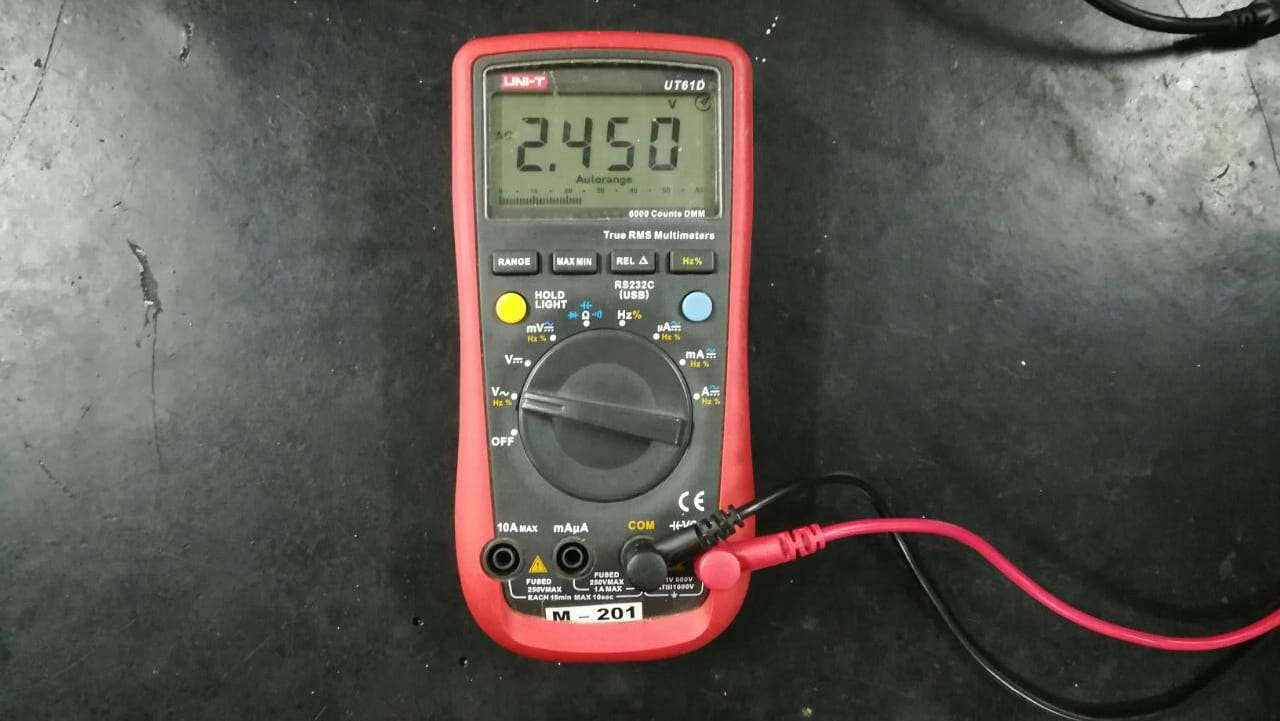
\includegraphics[width=\textwidth]{Imagenes/ActividadPractica/MedicionDeTensionEficaz/Exp1_Vrms_Cuadrada.jpeg}}
          \caption{Medición $V_{RMS}$.}
          \label{fig:MedicionVrmsCuadrada}
        \end{subfigure}
        \hfill 
        \begin{subfigure}[ht]{0.48\textwidth}
          \frame{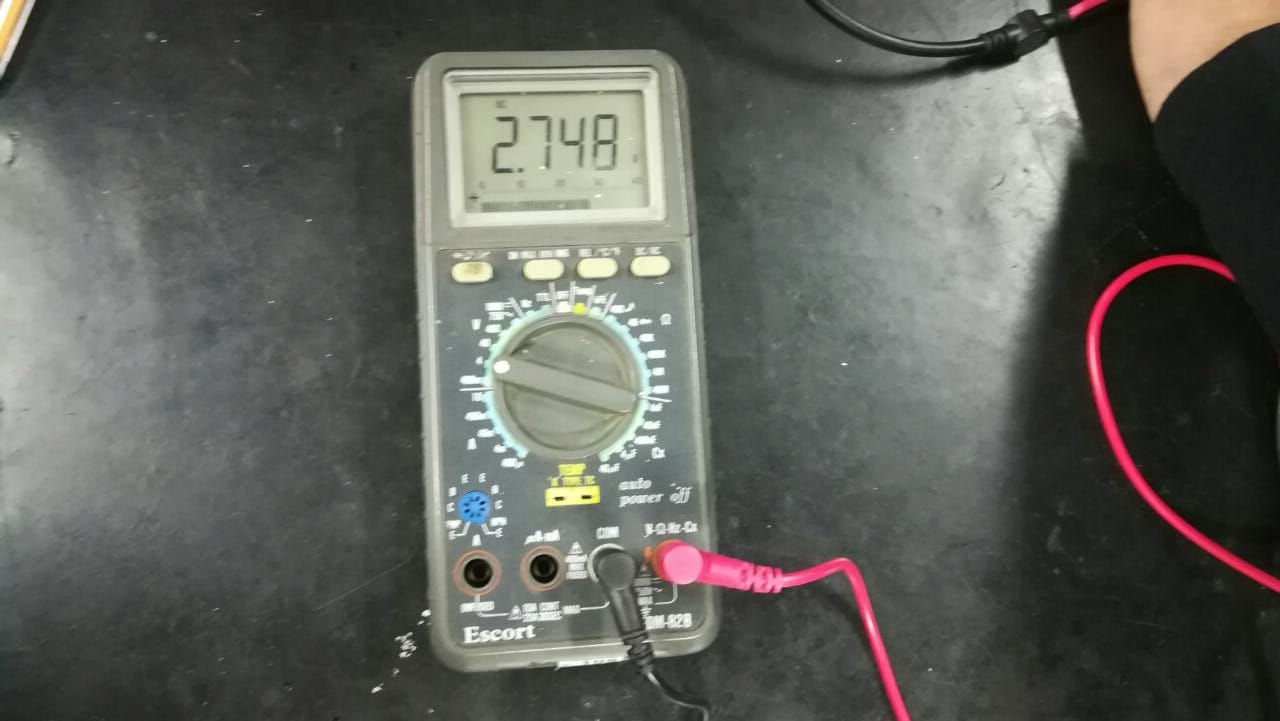
\includegraphics[width=\textwidth]{Imagenes/ActividadPractica/MedicionDeTensionEficaz/Exp1_Vmed_Cuadrada.jpeg}}
          \caption{Medición $V_{|med|}$.}
          \label{fig:MedicionVmedCuadrada}
        \end{subfigure}
        \caption{Mediciones de la señal cuadrada.}
         \label{fig:MedicionSeñalCuadrada}
      \end{figure}


      Luego, la cota de corrección para el multímetro de respuesta al valor medio del módulo es

      \begin{align*}
        e [\%] = \dfrac{V_{RMS} - V_{|med|}}{V_{|med|}} \cdot 100
               = \dfrac{2,450~V - 2,748~V}{2,748V} \cdot 100
               \hspace{20pt} \Longrightarrow \hspace{20pt} \Aboxed{e = -10,84\%}~.
      \end{align*}


    \subsubsection{En una onda triangular}
      En la Figura~\ref{fig:SeñalTriangular} se puede observar la señal triangular seteada.
      Luego, en la Figura~\ref{fig:MedicionSeñalTriangular} se observa la medición de tensión
      con ambos multímetros.

      \begin{figure}[H]
        \centering
        \frame{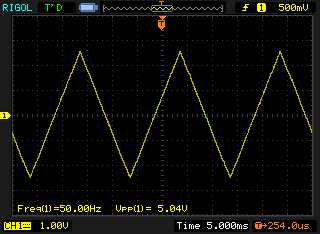
\includegraphics[width=0.45\textwidth]{Imagenes/ActividadPractica/MedicionDeTensionEficaz/Exp1_OndaTriangular.png}}
        \caption{Señal triangular a medir.}
        \label{fig:SeñalTriangular}
      \end{figure}

      \begin{figure}[H]
        \centering
        \begin{subfigure}[ht]{0.48\textwidth}
          \frame{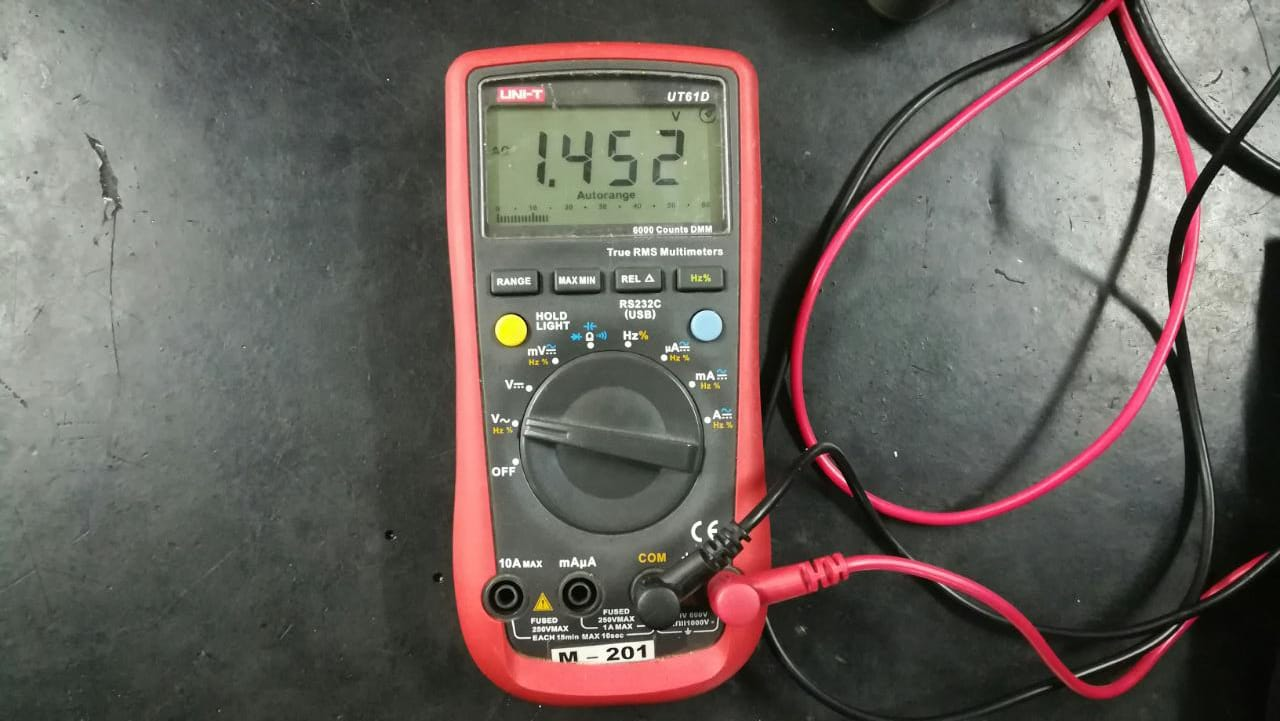
\includegraphics[width=\textwidth]{Imagenes/ActividadPractica/MedicionDeTensionEficaz/Exp1_Vrms_Triangular.jpeg}}
          \caption{Medición $V_{RMS}$.}
          \label{fig:MedicionVrmsTriangular}
        \end{subfigure}
        \hfill 
        \begin{subfigure}[ht]{0.48\textwidth}
          \frame{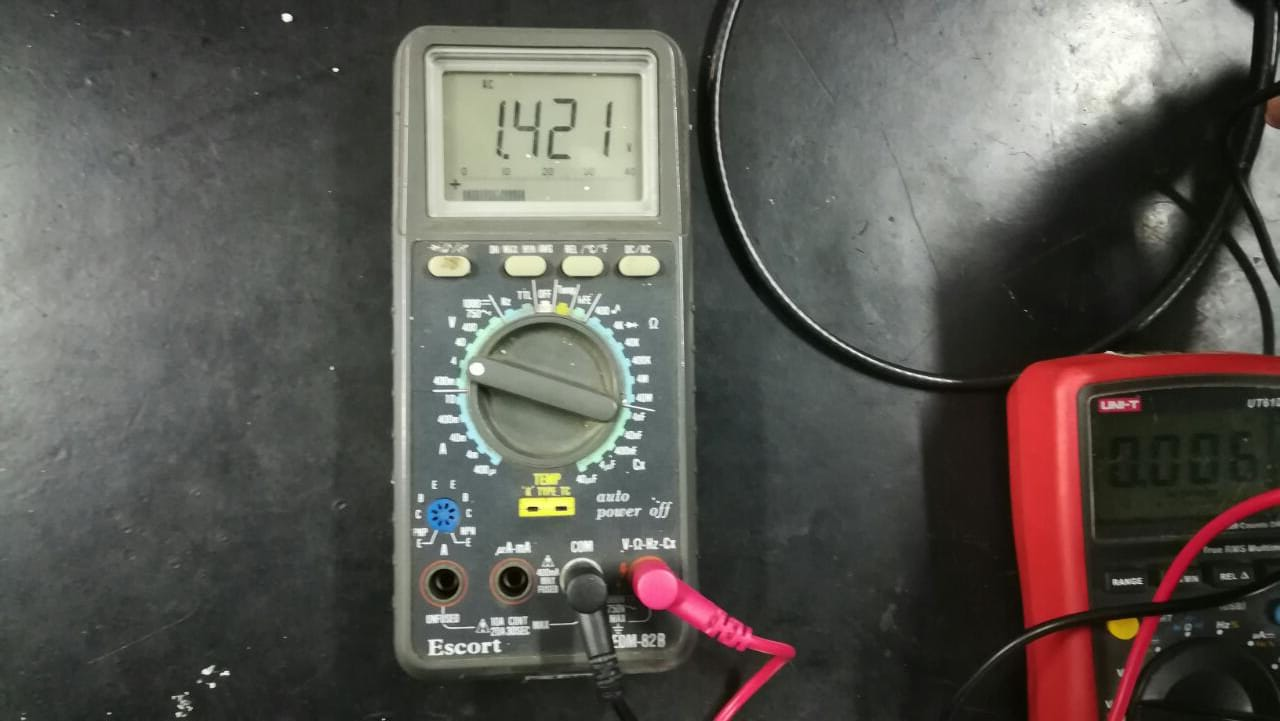
\includegraphics[width=\textwidth]{Imagenes/ActividadPractica/MedicionDeTensionEficaz/Exp1_Vmed_Triangular.jpeg}}
          \caption{Medición $V_{|med|}$.}
          \label{fig:MedicionVmedTriangular}
        \end{subfigure}
        \caption{Mediciones de la señal triangular.}
         \label{fig:MedicionSeñalTriangular}
      \end{figure}

      Luego, la cota de corrección para el multímetro de respuesta al 
      valor medio del módulo es

      \begin{align*}
        e [\%] = \dfrac{V_{RMS} - V_{|med|}}{V_{|med|}} \cdot 100
               = \dfrac{1,452~V - 1,421~V}{1,421~V} \cdot 100
               \hspace{20pt} \Longrightarrow \hspace{20pt} \Aboxed{e = +2,18\%}~.
      \end{align*}

    Los resultados de este experimento se encuentran consignados en la
    Tabla~\ref{tab:MedicionesOndasCuadYTrian}.
  
    \begin{table}[H] \centering
      \begin{tabular}{|c|c|c|c|} \hline
        \textbf{Señal}     & \textbf{Lectura RMS [V]}  & \textbf{Lectura |med| [V]} & \textbf{e [\%]} \\ \hline
      $\mathbf{Cuadrada~(50~Hz - 5~V_{pp})}$    & 2,450     & 2,748         &  -10,84        \\ \hline
      $\mathbf{Triangular~(50~Hz - 5~V_{pp})}$  & 1,452      & 1,421        &  +2,18         \\ \hline
      \end{tabular}
      \caption{Tabla de mediciones y cotas de corrección.}
      \label{tab:MedicionesOndasCuadYTrian}
    \end{table}
